% !TEX root = ../paper_zh.tex

\section{实验结果}

\subsection{成对红外-可见光单应性证据}

在 UAV-TAlign-12K 上，成对红外-可见光单应性证据整体具有很高可用性。
表~\ref{tab:pairwise_baselines_zh} 报告完整的 6,037 对正式评测划分。SIFT 和 AKAZE 作为经典
关键点参考，单应性可用率分别达到 87.08\% 和 94.29\%。RIFT2、raw MINIMA 和 RoMa 在每一对
评测图像上均能产生单应性，而 LoFTR 与 XoFTR 的可用率均超过 99\%。这些结果表明，红外专用
方法和现代稠密匹配器均可作为场景级对齐的强证据生成器。

\begin{table}[H]
\caption{UAV-TAlign-12K 上的成对红外-可见光单应性证据。单应性可用率表示鲁棒估计成功的
记录比例，其余列分别刻画声明部署配置下的对应关系支撑、空间范围、拟合残差和运行时间。}
\label{tab:pairwise_baselines_zh}
\centering
\resizebox{\textwidth}{!}{
\begin{tabular}{llrrrrrr}
\toprule
方法 & 类别 & OK / N $\uparrow$ & H (\%) $\uparrow$ & 内点率 $\uparrow$ & 覆盖率 $\uparrow$ & 重投影中位数 $\downarrow$ & 单对时间 (s) $\downarrow$ \\
\midrule
SIFT + RANSAC & 经典关键点 & 5257/6037 & 87.08 & 0.242 & 0.627 & 0.000 & 4.421 \\
AKAZE + RANSAC & 经典关键点 & 5692/6037 & 94.29 & 0.160 & 0.730 & 0.105 & 1.103 \\
RIFT2 (Python, resize-aware) & 红外-可见光经典方法 & 6037/6037 & \textbf{100.00} & 0.086 & 0.354 & 0.121 & 13.980 \\
raw MINIMA & 现代稠密 / 学习型 & 6037/6037 & \textbf{100.00} & 0.319 & 1.000 & 1.773 & 1.346 \\
RoMa outdoor & 现代稠密 / 学习型 & 6037/6037 & \textbf{100.00} & 0.328 & 0.997 & 1.741 & 0.929 \\
Kornia LoFTR outdoor (resize-aware) & 现代稠密 / 学习型 & 5984/6037 & 99.12 & 0.074 & 0.895 & 0.823 & 0.169 \\
XoFTR-640 & 现代稠密 / 学习型 & 5989/6037 & 99.20 & 0.089 & 0.949 & 1.732 & 0.647 \\
\bottomrule
\end{tabular}}
\end{table}

不同方法族呈现互补的证据特性。RIFT2 同时实现完整单应性可用率和较低拟合重投影误差，而 raw
MINIMA 与 RoMa 提供接近完整的空间覆盖。可用性、支撑度和覆盖率共同构成场景级基准轨道的
几何背景。

\begin{figure}[t]
\centering
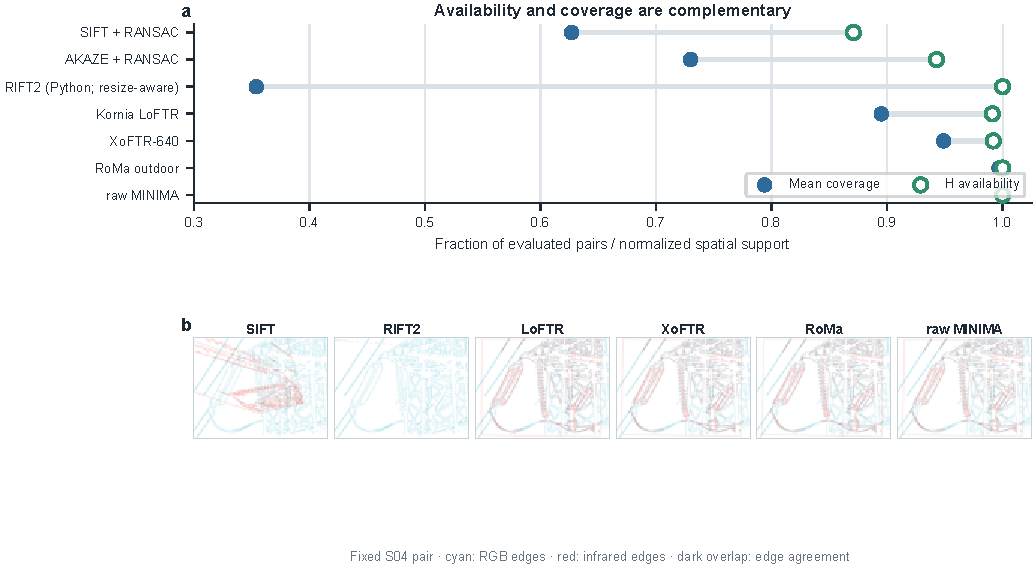
\includegraphics[width=\textwidth]{figures/fig05_pairwise_evidence.pdf}
\caption{不同匹配器家族的成对单应性证据。（a）单应性可用率与平均空间覆盖率从互补角度刻画
6,037 对正式评测划分上的证据完整性；（b）固定图像对的青色/红色边缘叠加，对比统一下游估计器
下代表性经典与学习型匹配器产生的几何支撑。}
\label{fig:pairwise_evidence_zh}
\end{figure}

\subsection{场景级参考结果}

UAV-TAlign 将成对证据转化为全部 15 个场景的变换。在规范运行点，框架识别出 9 个高置信产品，
对应 60.0\% 的场景覆盖率和 74.4\% 的图像对覆盖率。这些产品内部的接受帧支撑为 1491/2304
（64.7\%）。

\begin{table}[H]
\caption{UAV-TAlign 在 UAV-TAlign-12K 上的规范场景级运行点。图像对覆盖率和接受帧支撑均在
9 个高置信场景产品上计算。}
\label{tab:scene_level_main_zh}
\centering
\resizebox{\textwidth}{!}{
\begin{tabular}{llrrrrrr}
\toprule
方法 & 评测单位 & H 可用 $\uparrow$ & 高置信场景 $\uparrow$ & 场景覆盖率 (\%) $\uparrow$ & 图像对覆盖率 (\%) $\uparrow$ & 接受 / 尝试 & 接受率 (\%) $\uparrow$ \\
\midrule
UAV-TAlign & 15 个场景 & 15/15 & 9/15 & 60.0 & 74.4 & 1491/2304 & 64.7 \\
\bottomrule
\end{tabular}}
\end{table}

图~\ref{fig:scene_products_zh} 展示代表性规范对齐产品，覆盖不同光照、红外渲染和视图条件。统一
裁剪区域和边缘一致性视图使跨模态几何改善能够被直接检查。

\begin{figure}[t]
\centering
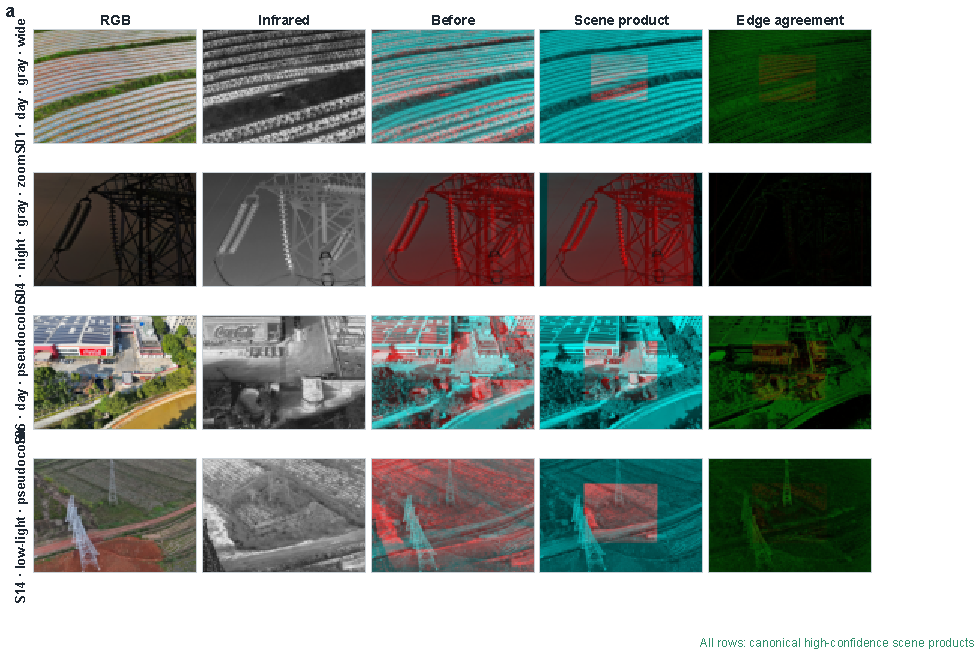
\includegraphics[width=\textwidth]{figures/fig06_scene_products.pdf}
\caption{规范运行点下的代表性 UAV-TAlign 高置信场景产品。各行覆盖白天、夜间与低照度场景，
并包含灰度和设备原生伪彩红外渲染；各列依次展示 RGB 裁剪、红外裁剪、未对齐叠加、场景单应性
叠加和边缘一致性可视化。}
\label{fig:scene_products_zh}
\end{figure}

\subsection{条件感知运行曲线}

不同光照条件呈现不同的场景产品和接受支撑特性。白天采集具有最高的场景覆盖率和接受帧比例；
夜间采集得到 3/5 个高置信产品；低照度采集在 3 个场景中保持 61.3\% 的接受帧比例。这两类互补
测量将可用帧支撑与最终场景产品区分开来。

\begin{table}[H]
\caption{按光照条件统计的运行曲线。接受/尝试表示每种条件下所有场景的汇总帧支撑。}
\label{tab:light_condition_zh}
\centering
\resizebox{\textwidth}{!}{
\begin{tabular}{lrrrrr}
\toprule
条件 & 场景数 & 高置信场景 $\uparrow$ & 场景覆盖率 (\%) $\uparrow$ & 接受 / 尝试 $\uparrow$ & 接受率 (\%) $\uparrow$ \\
\midrule
白天 & 7 & \textbf{5} & \textbf{71.4} & \textbf{1650/2203} & \textbf{74.9} \\
夜间 & 5 & 3 & 60.0 & 361/890 & 40.6 \\
低照度 & 3 & 1 & 33.3 & 462/754 & 61.3 \\
\bottomrule
\end{tabular}}
\end{table}

图~\ref{fig:operating_profile_zh}c,d 将分析扩展到光照、红外渲染与视图类型，同时报告场景保留率
和接受帧支撑。

\subsection{可靠性控制的场景选择}

匹配场景对照说明了为何成对支撑不能单独决定最终产品集合。图~\ref{fig:reliability_selection_zh}
在相同输出视图下比较广角/变焦和夜间对照，并将全部 15 个场景投影到接受支撑与严重离群点空间。
规范产品集中在低离群区域，而接受帧比例横跨保留场景与质量过滤场景。

\begin{figure}[t]
\centering
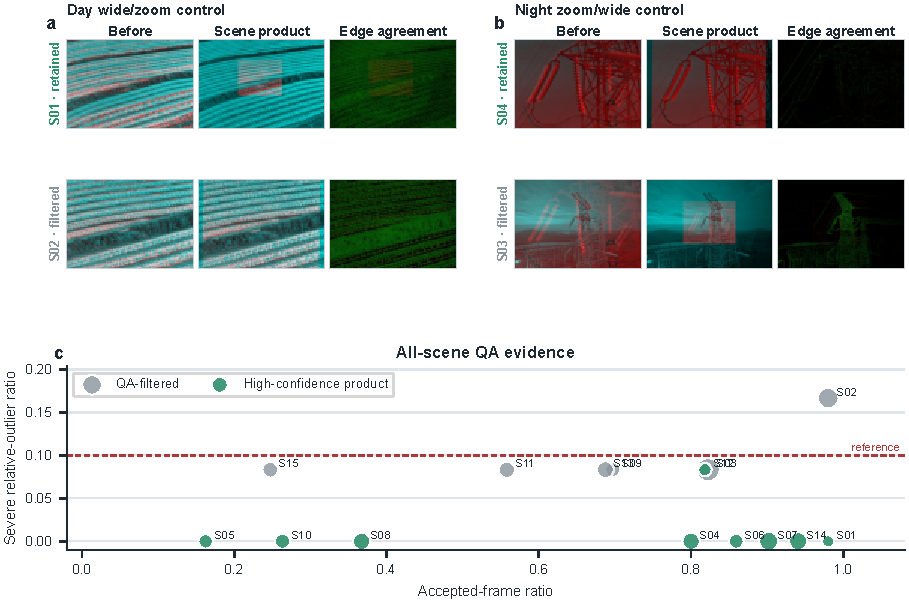
\includegraphics[width=\textwidth]{figures/fig07_reliability_selection.pdf}
\caption{匹配场景条件下的可靠性控制选择。（a,b）广角/变焦与夜间成对对照表明，较强成对支撑仍可
对应不同的规范场景结果；（c）在全部 15 个场景中，规范产品集中于较低严重离群点区域，而接受帧
比例不能单独决定保留结果。标记大小表示鲁棒剔除比例。}
\label{fig:reliability_selection_zh}
\end{figure}

\subsection{可靠性--覆盖率运行曲线}

固定的跨模态验证规则定义规范产品集合，可解释分数则对场景排序以形成连续的可靠性--覆盖率扫描。
图~\ref{fig:operating_profile_zh} 绘制基于分数排序的曲线，并叠加固定的规范运行点。

\begin{figure}[t]
\centering
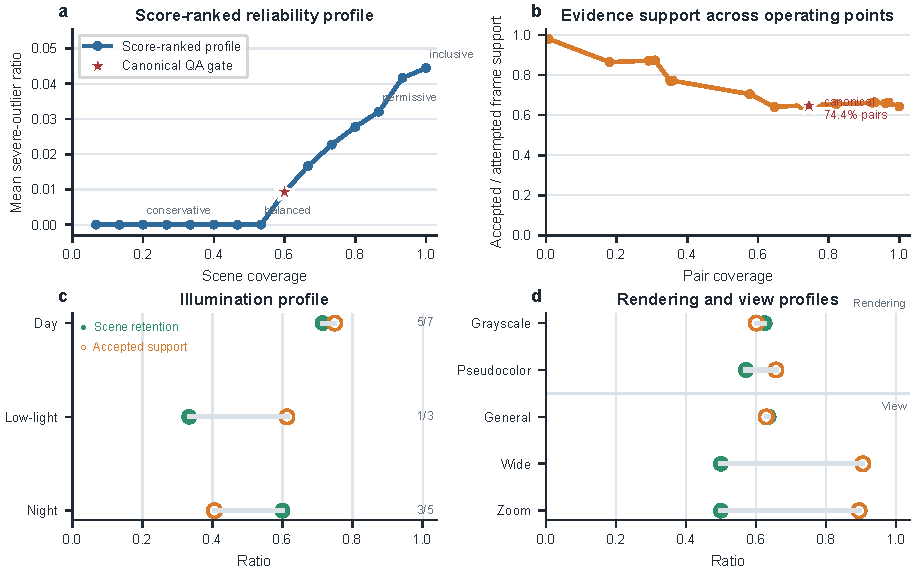
\includegraphics[width=\textwidth]{figures/fig08_operating_profile.pdf}
\caption{UAV-TAlign-12K 上的可靠性--覆盖率运行曲线。（a）基于分数排序的曲线刻画场景覆盖率提高
时的平均严重离群点比例，星号表示独立的规范 QA 运行点，而非分数排序的前九场景；（b）图像对
覆盖率和接受帧支撑给出相应证据范围；（c,d）条件感知曲线汇总光照、红外渲染与视图类型。}
\label{fig:operating_profile_zh}
\end{figure}

在规范运行点，UAV-TAlign 识别出 9 个高置信产品，覆盖 60.0\% 的场景和 74.4\% 的评测图像对，
平均严重离群点比例为 0.009。基于分数排序的曲线提供了从高置信运行到更广覆盖范围的平滑过渡。
图~\ref{fig:operating_profile_zh} 中的规范点对应 9/15 个场景、60.0\% 场景覆盖率和 74.4\% 图像对
覆盖率。

\subsection{场景诊断的受控验证}

场景诊断量在独立重采样和受控几何扰动下表现出一致响应。五折留帧分析覆盖全部 15 个场景和
75 次共识重计算。每折留出约五分之一的接受帧假设时，相对完整证据共识的位移中位数为 1.39
像素，平均值为 2.26 像素。

扰动实验覆盖 45 个代表帧和 675 次受控试验。在每一种扰动类型中，随严重度提高，联合边缘/梯度
质量信号均单调下降。在最大扰动严重度下，平移、旋转和尺度扰动引起的平均联合分数变化分别为
$-0.074$、$-0.031$ 和 $-0.025$，相应退化比例为 84.4\%、80.0\% 和 73.3\%。
表~\ref{tab:protocol_validation_zh} 汇总了这些独立证据。
图~\ref{fig:validation_attribution_zh}a,b 进一步展示逐场景重采样响应和随扰动强度变化的质量趋势。

\begin{table}[H]
\caption{场景共识稳定性与跨模态质量敏感性的受控验证。合成退化比例和联合分数变化均在最大测试
严重度下报告。}
\label{tab:protocol_validation_zh}
\centering
\resizebox{0.92\textwidth}{!}{
\begin{tabular}{llrr}
\toprule
验证方式 & 范围 & 主要响应 & 退化试验 (\%) \\
\midrule
留帧共识 & 15 个场景 / 75 折 & 1.39 px 场景中位漂移 & -- \\
合成平移 & 45 帧 / 225 次试验 & $\Delta$Joint $=-0.074$ & 84.4 \\
合成旋转 & 45 帧 / 225 次试验 & $\Delta$Joint $=-0.031$ & 80.0 \\
合成尺度 & 45 帧 / 225 次试验 & $\Delta$Joint $=-0.025$ & 73.3 \\
\bottomrule
\end{tabular}}
\end{table}

\subsection{累加式消融实验}

固定 8 场景消融用于分离鲁棒共识和跨模态验证的作用。鲁棒共识将平均边缘增益从 0.124 提高到
0.146，将梯度 NCC 增益从 0.126 提高到 0.149；同时，严重离群点比例从 0.104 降至 0.042，
变换离散度从 151.2 像素降至 52.5 像素。跨模态验证进一步把阶段输出映射为规范产品决策。

\begin{table}[H]
\caption{固定 8 场景 UAV-TAlign-1K-Lite 子集上的累加式消融。}
\label{tab:ablation_main_zh}
\centering
\resizebox{\textwidth}{!}{
\begin{tabular}{lcccrrrrr}
\toprule
变体 & 选择 & 共识 & 验证 & 阶段通过/N $\uparrow$ & $\Delta$Edge $\uparrow$ & $\Delta$Grad $\uparrow$ & Severe $\downarrow$ & Disp. (px) $\downarrow$ \\
\midrule
仅成对证据 & even & \xmark & \xmark & 8/8 & 0.124 & 0.126 & 0.104 & 151.2 \\
+ 鲁棒场景共识 & even & \cmark & \xmark & 8/8 & 0.146 & 0.149 & 0.042 & 52.5 \\
+ 跨模态验证 & even & \cmark & \cmark & 5/8 & 0.146 & 0.148 & 0.042 & 57.7 \\
\bottomrule
\end{tabular}}
\end{table}

图~\ref{fig:validation_attribution_zh}c,d 将累加式模块效应与多随机种子选择分析联系起来：鲁棒共识
贡献最大的诊断增益，而确定性调度提供稳定的参考运行策略。

\begin{figure}[t]
\centering
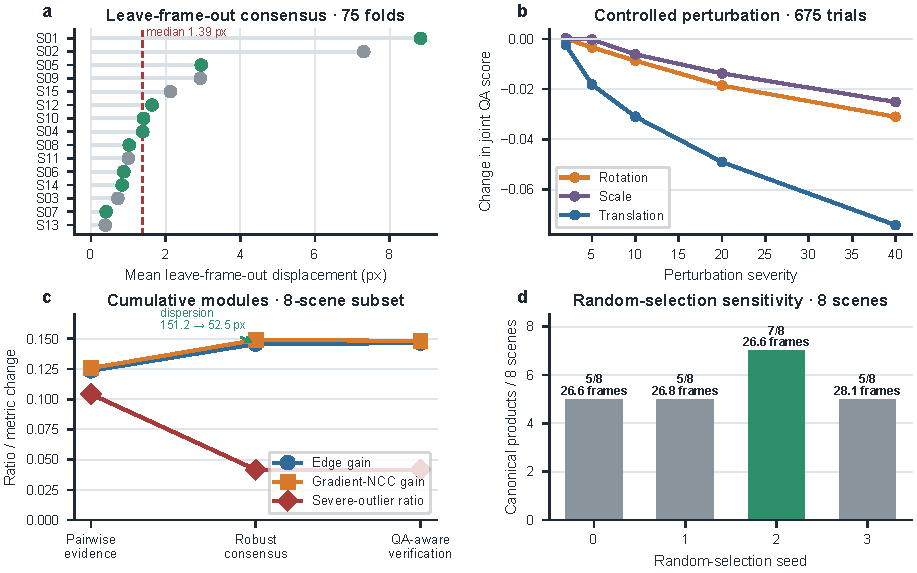
\includegraphics[width=\textwidth]{figures/fig09_validation_attribution.pdf}
\caption{受控验证与模块归因。（a）全部 15 个场景上的五折留帧共识；（b）随平移、旋转与尺度扰动
增强而变化的联合边缘/梯度质量；（c）固定八场景诊断子集上的累加式模块效应；（d）同一子集上
不同随机种子的选择敏感性。}
\label{fig:validation_attribution_zh}
\end{figure}

在不同随机选择种子下，同一固定子集得到 5/8 至 7/8 个场景产品，而平均接受帧支撑保持相对稳定。
该结果确认确定性均匀选择是一种可复现的运行策略，并将随机种子敏感性定位于少量接近阈值的场景。
